\begin{frame}[noframenumbering]
\Large{\textbf{Appendices}}
\end{frame}


\begin{frame}[noframenumbering]
\Large{\textbf{Bernstein-Bézier properties}}
\end{frame}





\begin{frame}[noframenumbering]{Bernstein-Bézier polynomial basis}
\vspace{-0.2cm}
\scriptsize
\begin{block}{\scriptsize{Polynomial basis expression:}}
In an arbitrary dimension, $\balpha \in \mathbb{N}^{\dim+1}$ with $\sum_{i=0}^N \alpha_i = N$
and $\blambda \in [0,1]^{\dim+1}$ with $\sum_{i=0}^N \hat{\lambda}_i = 1$.
For example, we have in 3D the following notation:
\begin{equation}
        B^\PolOrder_\balpha(\blambda) = B^\PolOrder_{ijkl}(\lzero,\lone,\ltwo,\lthree) = C^\PolOrder_{ijkl} \lzero^i \lone^j \ltwo^k \lthree^l = \frac{\PolOrder!}{i!j!k!l!}\lzero^i \lone^j \ltwo^k \lthree^l
\end{equation}
\end{block}
\vspace{-0.1cm}
\uncover<2->{
\begin{block}{\scriptsize{Property 1: Sparse elevation order}}
A Bernstein polynomial of order $N-1$
can be represented with a linear combination of $\dim+1$ Bernstein polynomials
of order $\PolOrder$ as follows:

\begin{equation}
B^{\PolOrder-1}_\balpha(\blambda) = \sum_{i=0}^\dim \frac{\alpha_i+1}{\PolOrder} B^\PolOrder_{\balpha + \ecan_i}(\blambda)\,. \label{elev_order_bb}
\end{equation}
\end{block}
}
\vspace{-0.1cm}
\uncover<3->{
\begin{block}{\scriptsize{Property 2: Sparse dervative operator}}
The derivative of a Bernstein polynomial $B^\PolOrder_\balpha$ with respect to $\hat{\lambda}_i$ is given by:
\begin{equation}
\frac{\partial B^\PolOrder_\balpha}{\partial \hat{\lambda}_i} (\blambda)= N B^{\PolOrder-1}_{\balpha-\ecan_i} (\blambda)\,.
\end{equation}
\end{block}
}
\end{frame}



\begin{frame}[noframenumbering]
\Large{\textbf{WADG formula}}
\end{frame}



\begin{frame}[noframenumbering]{Weight Adjusted Discontinuous Galerkin (WADG)}
  \scriptsize

  \begin{equation}
(\Mass^\element_\param)^{-1} \approx (\Mwadg^\element_\param)^{-1} = (\Mass^\element)^{-1} \Mass^\element_{1/\param} (\Mass^\element)^{-1}
\label{inv_wadg}
\end{equation}
\begin{equation}
\Mass^\element_{\frac{1}{\param}} = \detJK \, \Pquad\, diag(\weight \frac{1}{\coefParam^\element})\, \Pquad^\top \label{wadg_operator}
\end{equation}


\begin{itemize}
\item $\coefParam^\element$: vector of size $\nquad$;
\item $\Pquad$: Matrix of size $\dof \times \nquad$ such as $[Q]_{i,q} = \hat{\varphi_i}(\refx_q)$\,;
\item $diag(\weight \frac{1}{\coefParam^\element})$: diagonal matrix of size $\nquad \times \nquad$ where $diag(\weight \frac{1}{\coefParam})_{q,q} = \sweight_q \frac{1}{\coefParam^\element_q}$\,.
\item $\detJK$: Determinant of the Jacobian of the transformation from $\element$ to the reference element.
\end{itemize}

\uncover<2->{
\tiny
\begin{empheq}[left=\empheqlbrace]{align}
  & \frac{\partial \textcolor{\myred}{\coefPolP}^\element}{\partial t}
    = -  \MassRef^{-1} \, \Pquad\, diag(\weight \boldsymbol{\bm}^\element)\, \Pquad^\top  \left( \sum_{k=1}^\dim \sum_{d=1}^\dim [J_{T_\element}^{-\top}]_{k,d} \MassRef^{-1}\StiffRef_\refxd \textcolor{\myred}{\coefPolVd}
  -  \sum_{d=1}^\dim \sum_{\Edge \in \element} \frac{\detJF}{\detJK} \MassRef^{-1}\MassRef_\Edge \textcolor{\myred}{\FluxP}^\Edge \right)
  +  \coefpolSource^\element  \\
  & \frac{\partial \textcolor{\myred}{\coefPolVd}^\element}{\partial t} =
  -  \MassRef^{-1} \, \Pquad\, diag(\weight \boldsymbol{\frac{1}{\density}}^\element)\, \Pquad^\top  \left( \sum_{k=1}^\dim [J_{T_\element}^{-\top}]_{k,d} \MassRef^{-1}\StiffRef_\refxd \textcolor{\myred}{\coefPolP}^\element
  - \sum_\Edge \frac{\detJF}{\detJK} \MassRef^{-1}\MassRef_\Edge \textcolor{\myred}{\FluxV}_d^\Edge \right)\,,
  \label{semi_discrete_wadg_operator}
\end{empheq}
for $d=1\,\,\text{to}\,\,\dim$ \hfill.
}
\end{frame}


\begin{frame}{WADG small experiment}

  \setlength{\modelwidth}{6.0cm}
\begin{figure}[htbp]
\begin{subfigure}{1.0\textwidth}
  \renewcommand{\modelfile}{image/num_exp_1/bicouche_model}
     \renewcommand{\cmapmin}{1500}
     \renewcommand{\cmapmax}{3000}
     \centering
     \begin{tikzpicture}
\pgfmathsetmacro{\xmin} {0.}
\pgfmathsetmacro{\xmax} {9.7}
\pgfmathsetmacro{\zmin} {0.}
\pgfmathsetmacro{\zmax} {2.7}
\pgfmathsetmacro{\zzmax} {3.0}
\pgfmathsetmacro{\xxmax} {10.0}


\begin{axis}[%
width=1.0\modelwidth,
height=0.5\modelwidth,
axis on top, separate axis lines,
xmin=\xmin, xmax=\xxmax, %xlabel={x (km)},
ymin=\zmin, ymax=\zzmax,
yticklabels={},xticklabels={},
y dir=reverse,
colormap/paraview, colorbar,
colorbar style={title=\small{$m \cdot s^{-1}$}},
point meta min=\cmapmin, point meta max=\cmapmax,
colorbar/width=2.5mm,
axis x line=top,thick,
axis y line=left,thick,
ylabel style={rotate=-90},
ylabel={$z$},
xlabel={$x$},
ticks = none,
]
\addplot [forget plot] graphics [xmin=\xmin,xmax=\xmax,ymin=\zmin,ymax=\zmax] {{\modelfile}.png};
\end{axis}
\end{tikzpicture}%

     \caption{Bi-layered wavespeed model (reference).}
     \label{bicouche_model_with_mesh}
\end{subfigure}

\begin{subfigure}{0.45\textwidth}
  \renewcommand{\modelfile}{image/num_exp_1/bicouche_p4q1}
     \renewcommand{\cmapmin}{1500}
     \renewcommand{\cmapmax}{3000}
     \centering
     \begin{tikzpicture}
  \pgfmathsetmacro{\xmin} {0.}
\pgfmathsetmacro{\xmax} {9.7}
\pgfmathsetmacro{\zmin} {0.}
\pgfmathsetmacro{\zmax} {2.7}
\pgfmathsetmacro{\zzmax} {3.0}
\pgfmathsetmacro{\xxmax} {10.0}

\begin{axis}[%
width=1.0\modelwidth,
height=0.5\modelwidth,
axis on top, separate axis lines,
xmin=\xmin, xmax=\xxmax, %xlabel={x (km)},
ymin=\zmin, ymax=\zzmax,
yticklabels={},xticklabels={},
y dir=reverse,
point meta min=1.5e3, point meta max=5.5e3,
axis x line=top,thick,
axis y line=left,thick,
ylabel style={rotate=-90},
ylabel={$z$},
xlabel={$x$},
ticks = none,
]
\addplot [forget plot] graphics [xmin=\xmin,xmax=\xmax,ymin=\zmin,ymax=\zmax] {{\modelfile}.png};
\end{axis}
\end{tikzpicture}%

     \caption{Bi-layered wavespeed model (P4 Q1).}
     \label{bicouche_model_without_mesh}
\end{subfigure}
\hspace{0.5cm}
\begin{subfigure}{0.45\textwidth}
  \renewcommand{\modelfile}{image/num_exp_1/bicouche_p4q9}
     \renewcommand{\cmapmin}{1500}
     \renewcommand{\cmapmax}{3000}
     \centering
     \begin{tikzpicture}
  \pgfmathsetmacro{\xmin} {0.}
\pgfmathsetmacro{\xmax} {9.7}
\pgfmathsetmacro{\zmin} {0.}
\pgfmathsetmacro{\zmax} {2.7}
\pgfmathsetmacro{\zzmax} {3.0}
\pgfmathsetmacro{\xxmax} {10.0}

\begin{axis}[%
width=1.0\modelwidth,
height=0.5\modelwidth,
axis on top, separate axis lines,
xmin=\xmin, xmax=\xxmax, %xlabel={x (km)},
ymin=\zmin, ymax=\zzmax,
yticklabels={},xticklabels={},
y dir=reverse,
point meta min=1.5e3, point meta max=5.5e3,
axis x line=top,thick,
axis y line=left,thick,
ylabel style={rotate=-90},
ylabel={$z$},
xlabel={$x$},
ticks = none,
]
\addplot [forget plot] graphics [xmin=\xmin,xmax=\xmax,ymin=\zmin,ymax=\zmax] {{\modelfile}.png};
\end{axis}
\end{tikzpicture}%

     \caption{Bi-layered wavespeed model (P4 Q9).}
     \label{bicouche_model_with_wadg}
\end{subfigure}
\caption{Illustration of the wavespeed model for three different configurations.}
\label{bicouche_meshes}
\end{figure}
\end{frame}


\begin{frame}[noframenumbering]{WADG small experiment}
\vspace{-0.3cm}
\begin{figure}[htbp]
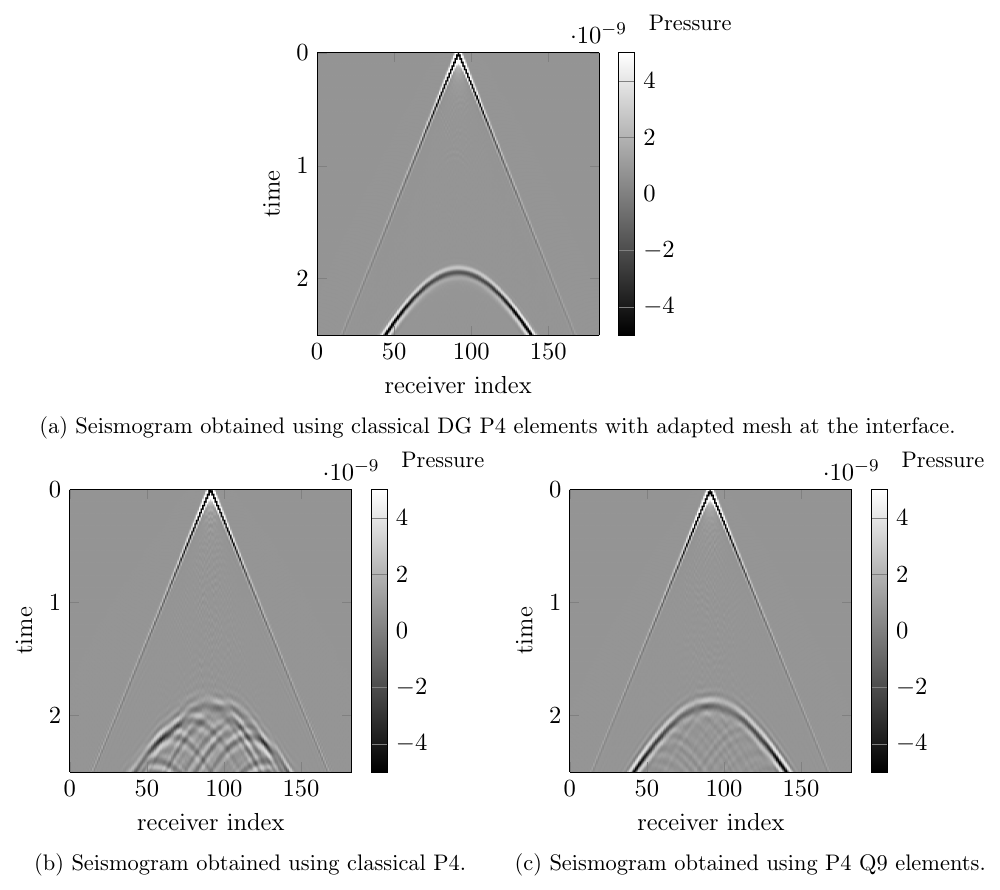
\includegraphics[scale=0.25]{image/flemme_wadg.png}
\end{figure}


\end{frame}








\begin{frame}[noframenumbering]

\Large{\textbf{Interface refinement}}

\end{frame}


\begin{frame}[noframenumbering]{Influence of the cloud point on the gradient}
\begin{figure}[H]
\centering
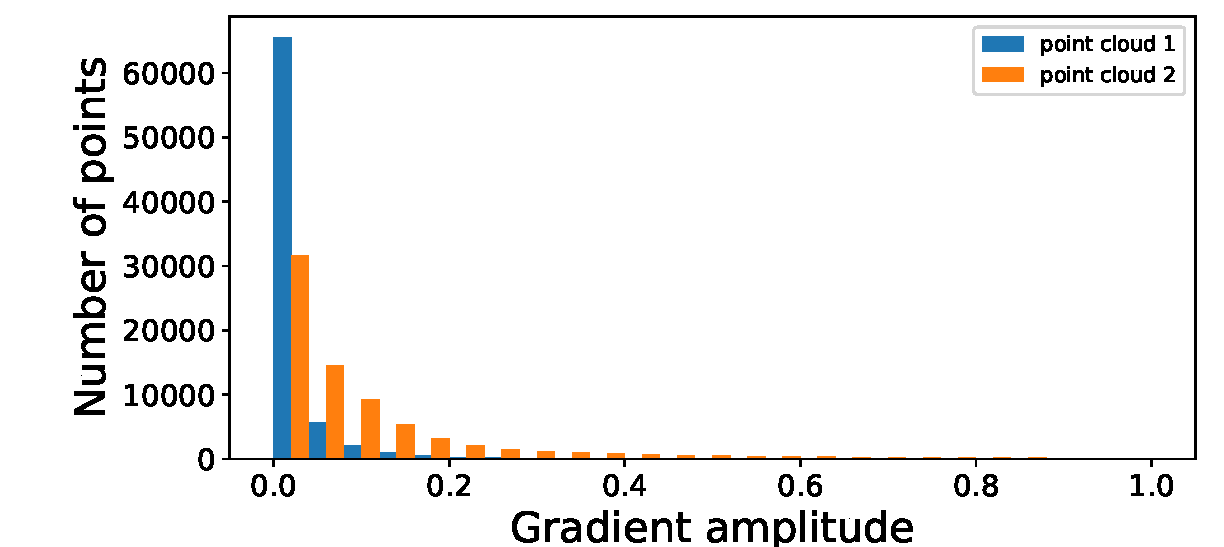
\includegraphics[scale=0.5]{image/histo_comparison_grad.pdf}
\caption{Histogram recording the number of points in the
point cloud as a function of the normalized gradient amplitude for two different point clouds.}
\label{histo_comparison_grad}
\end{figure}
\end{frame}



\begin{frame}[noframenumbering]{Influence of epsilon of the interface detection}
  \small
\setlength{\modelwidth}{6.1cm}
\begin{figure}[!htbp]
\renewcommand{\cmapmin}{0}
\renewcommand{\cmapmax}{1}
\renewcommand{\modelfile}{image/mesh_adapt/interface_tresh_02}
\begin{subfigure}{0.5\textwidth}
\vspace{0.0cm}
\centering
\begin{tikzpicture}
\pgfmathsetmacro{\xmin} {0.}
\pgfmathsetmacro{\xmax} {9.7}
\pgfmathsetmacro{\zmin} {0.}
\pgfmathsetmacro{\zmax} {2.7}
\pgfmathsetmacro{\zzmax} {3.0}
\pgfmathsetmacro{\xxmax} {10.0}

\begin{axis}[%
width=1.0\modelwidth,
height=0.5\modelwidth,
axis on top, separate axis lines,
xmin=\xmin, xmax=\xxmax, %xlabel={x (km)},
ymin=\zmin, ymax=\zzmax,
yticklabels={},xticklabels={},
y dir=reverse,
point meta min=1.5e3, point meta max=4.6e3,
colorbar/width=2.5mm,
axis x line=top,thick,
axis y line=left,thick,
ylabel style={rotate=-90},
ylabel={$z$},
xlabel={$x$},
ticks = none,
]
\addplot [forget plot] graphics [xmin=\xmin,xmax=\xmax,ymin=\zmin,ymax=\zmax] {{\modelfile}.png};
\end{axis}
\end{tikzpicture}%

\caption{Interfaces highlighted using $\epsilon=0.2$.}
\end{subfigure}
\hspace{-0.5cm}
\renewcommand{\modelfile}{image/mesh_adapt/interface_tresh_01}
\begin{subfigure}{0.5\textwidth}
\centering
\begin{tikzpicture}
\pgfmathsetmacro{\xmin} {0.}
\pgfmathsetmacro{\xmax} {9.7}
\pgfmathsetmacro{\zmin} {0.}
\pgfmathsetmacro{\zmax} {2.7}
\pgfmathsetmacro{\zzmax} {3.0}
\pgfmathsetmacro{\xxmax} {10.0}


\begin{axis}[%
    width=1.0\modelwidth,
    height=0.5\modelwidth,
    axis on top, separate axis lines,
    xmin=\xmin, xmax=\xxmax, %xlabel={x (km)},
    ymin=\zmin, ymax=\zzmax,
    yticklabels={},xticklabels={},
    y dir=reverse,
    colormap/jet, colorbar,
    point meta min=\cmapmin, point meta max=\cmapmax,
    colorbar/width=2.5mm,
    axis x line=top,thick,
    axis y line=left,thick,
    ylabel style={rotate=-90},
    ylabel={$z$},
    xlabel={$x$},
    ticks = none,
]
\addplot [forget plot] graphics [xmin=\xmin,xmax=\xmax,ymin=\zmin,ymax=\zmax] {{\modelfile}.png};
\end{axis}
\end{tikzpicture}%

\vspace{-0.7cm}
\caption{Interfaces highlighted using $\epsilon=0.1$.}
\end{subfigure}

\renewcommand{\modelfile}{image/grad_e}
\begin{subfigure}{0.5\textwidth}
\vspace{0.0cm}
\centering
\begin{tikzpicture}
\pgfmathsetmacro{\xmin} {0.}
\pgfmathsetmacro{\xmax} {9.7}
\pgfmathsetmacro{\zmin} {0.}
\pgfmathsetmacro{\zmax} {2.7}
\pgfmathsetmacro{\zzmax} {3.0}
\pgfmathsetmacro{\xxmax} {10.0}

\begin{axis}[%
width=1.0\modelwidth,
height=0.5\modelwidth,
axis on top, separate axis lines,
xmin=\xmin, xmax=\xxmax, %xlabel={x (km)},
ymin=\zmin, ymax=\zzmax,
yticklabels={},xticklabels={},
y dir=reverse,
point meta min=1.5e3, point meta max=4.6e3,
colorbar/width=2.5mm,
axis x line=top,thick,
axis y line=left,thick,
ylabel style={rotate=-90},
ylabel={$z$},
xlabel={$x$},
ticks = none,
]
\addplot [forget plot] graphics [xmin=\xmin,xmax=\xmax,ymin=\zmin,ymax=\zmax] {{\modelfile}.png};
\end{axis}
\end{tikzpicture}%

\caption{Interfaces highlighted using $\epsilon=0.08$.}
\end{subfigure}
\hspace{-0.5cm}
\begin{subfigure}{0.5\textwidth}
\centering
\renewcommand{\modelfile}{image/mesh_adapt/interface_tresh_002}
\begin{tikzpicture}
\pgfmathsetmacro{\xmin} {0.}
\pgfmathsetmacro{\xmax} {9.7}
\pgfmathsetmacro{\zmin} {0.}
\pgfmathsetmacro{\zmax} {2.7}
\pgfmathsetmacro{\zzmax} {3.0}
\pgfmathsetmacro{\xxmax} {10.0}


\begin{axis}[%
    width=1.0\modelwidth,
    height=0.5\modelwidth,
    axis on top, separate axis lines,
    xmin=\xmin, xmax=\xxmax, %xlabel={x (km)},
    ymin=\zmin, ymax=\zzmax,
    yticklabels={},xticklabels={},
    y dir=reverse,
    colormap/jet, colorbar,
    point meta min=\cmapmin, point meta max=\cmapmax,
    colorbar/width=2.5mm,
    axis x line=top,thick,
    axis y line=left,thick,
    ylabel style={rotate=-90},
    ylabel={$z$},
    xlabel={$x$},
    ticks = none,
]
\addplot [forget plot] graphics [xmin=\xmin,xmax=\xmax,ymin=\zmin,ymax=\zmax] {{\modelfile}.png};
\end{axis}
\end{tikzpicture}%

\vspace{-0.7cm}
\caption{Interfaces highlighted using $\epsilon=0.02$.}
\end{subfigure}
\caption{Marmousi highlighted interfaces for several threshold values.}
\label{interface_thresholds}
\end{figure}
\end{frame}


\begin{frame}[noframenumbering]{Modify the metric $\metric$ to deals with interface}
  if $Interface(P) = 1$

  \begin{multicols}{2}
    \large{\textbf{\textcolor{\mygreen}{Isotropic metric}}}
    \vspace{0.5cm}

    \uncover<2->{
    \small{In all direction:}
    \normalsize
    \begin{equation}
      \scriptstyle
      h(P) =  \frac{1}{r} 2\frac{\lambda(P)}{\nppw}\sqrt{\frac{(\PolOrder+1)(\PolOrder+2)}{2\sqrt{3}}},\, r\geq1.0
    \end{equation}
    \vfill
    }

    \columnbreak

    \large{\textbf{\textcolor{blue}{Anisotropic metric}}}
    \vspace{0.5cm}

    \uncover<3->{
    \small{In $\vec{\nabla} \velocity$ direction:}
    \normalsize
    \begin{equation}
      \scriptstyle
      hr(P) =  \frac{1}{r} 2\frac{\lambda(P)}{\nppw}\sqrt{\frac{(\PolOrder+1)(\PolOrder+2)}{2\sqrt{3}}},\, r\geq1.0
    \end{equation}

    \small{In $\vec{\nabla} \velocity^\top$ direction:}
    \normalsize
    \begin{equation}
      \scriptstyle
      h(P) =  2\frac{\lambda(P)}{\nppw}\sqrt{\frac{(\PolOrder+1)(\PolOrder+2)}{2\sqrt{3}}}.
    \end{equation}
    \vfill
    }

    \end{multicols}

\end{frame}


\begin{frame}[noframenumbering]

  \begin{multicols}{2}
    \large{\textbf{\textcolor{\mygreen}{Isotropic metric}}}

    \columnbreak

    \large{\textbf{\textcolor{blue}{Anisotropic metric}}}

  \end{multicols}

  \begin{table}[H]
    \small
\centering
\begin{tabular}{|l|l|l|l|l|l|l|l|}
\hline
& $\nbelem$  & $r$  & P2 & P3 & P4 &  CPU & Relative  \\
&  & &  &  &  & time(s) & L2 error \\ \hline
Mesh 1 &6808 &  1           &  <0.1\% & 8\% &92\% & 379 & 15.2\% \\ \hline
\rowcolor{green!30}
Mesh 2 &8434 &  $\sqrt{2}$  & 2\% & 25\% & 73\% & 463 & 10.5\% \\ \hline
\rowcolor{blue!30}
Mesh 2'&8226 &  $\sqrt{2}$  & 1\% & 14\% & 85\% & 602 & 8.5\% \\ \hline
\rowcolor{green!30}
Mesh 3 &12809&  2           & 24\% &62\% & 27\% & 815 & 5.2\% \\ \hline
\rowcolor{blue!30}
Mesh 3'&11496&  2           & 5\% & 37\% & 58\% & 1731 & 5.1\%  \\ \hline
Mesh 4 &26621&  ref.        & 0\% & 0\% & 100\% & 4384 & ref. \\ \hline
\end{tabular}
\caption{Performance comparison between isotropic and anisotropic mesh refinement.}
\label{mesh_iso_aniso_comp}
\end{table}
  \end{frame}



\begin{frame}[noframenumbering]{Modify the metric $\metric$ to deals with interface}


  \begin{multicols}{2}
        \large{\textbf{\textcolor{\mygreen}{Isotropic metric}}}
    \vspace{0.5cm}
    \begin{itemize}
      \item[\textcolor{\mygreen}{\textbf{+}}] Better capture the interfaces
      \item[\textcolor{\mygreen}{\textbf{+}}] Enhenced precision
      \item[\textcolor{\mygreen}{\textbf{+}}] Adapted for explicit time schemes
      \item[\textcolor{\myred}{\textbf{-}}] Have more $\dof$ for a lower accuracy
      \end{itemize}

    \columnbreak
    \large{\textbf{\textcolor{blue}{Anisotropic metric}}}
    \vspace{0.5cm}
    \begin{itemize}
      \item[\textcolor{\mygreen}{\textbf{+}}] Better capture the interfaces
      \item[\textcolor{\mygreen}{\textbf{++}}] Enhenced precision
      \item[\textcolor{\myred}{\textbf{- -}}] Not adapted for explicit time schemes
      \item[\textcolor{\mygreen}{\textbf{++}}] Get lower $\dof$ for a better accuracy
    \end{itemize}
  \end{multicols}

  \uncover<2->{
    \begin{block}{Warning}
      The refinement depends on the interface detection which is still an empirical selection ($\epsilon$).
    \end{block}
    }

\end{frame}
